%\documentclass[journal=jceaax,manuscript=article]{achemso}
\documentclass[11pt,reqno]{amsart}
\pagestyle{plain}
\usepackage{amsmath}
\usepackage{mathtools}
\usepackage{dcolumn}
\usepackage{multirow}

\usepackage{epsfig}
\usepackage{graphicx}
\usepackage{bm}        % for math
\usepackage{amssymb}   % for math
\usepackage{epstopdf}
\usepackage{geometry}                % See geometry.pdf to learn the layout options. There are lots.
\geometry{letterpaper}                   % ... or a4paper or a5paper or ... 
%\usepackage[parfill]{parskip}    % Activate to begin paragraphs with an empty line rather than an indent
\usepackage{amssymb}


\DeclareGraphicsRule{.tif}{png}{.png}{`convert #1 `dirname #1`/`basename #1 .tif`.png}

\title{Electric-field mapped averaging for non-interacting and interacting dipoles}
\author{W.L , D.A.K}
\date{}                                           % Activate to display a given date or no date

\begin{document}
\maketitle
\section{Non-interacting dipoles}
%\subsection{}
We first briefly review the formulation for ${\bf v}^{\bf E}$ for non-interacting dipoles (the case in our JCTC paper). The energy function for ideal dipoles under electric field is
\begin{equation}
\label{eq:noninteract}
u ={{\bf E} \cdot {\bf M}}= -E_z\mu\sum_i^N \cos\theta_i.
\end{equation}
$\mu$ is the dipole moment, ${\bf E}$ is the electric field and ${\bf M}=\sum_{i}{\boldsymbol \mu}_i$ is the the total dipole polarization obtained by summation of all the dipoles; the latter equality in \eqref{eq:noninteract} assumes that ${\bf E}$ has non-zero component in the $z$ direction only. For the mapping coordinate, we define $z_i = \cos\theta_i$, the $z$-component of the unit dipole vector of molecule $i$ as oriented in a given configuration, so $-1\le z_i \le 1$. An approximate $p(\boldsymbol\mu,{\bf E})$ is formed from this energy function. Specifically, we identify $p_1(z_i,{E}_z) = \exp\left(\beta\mu { E}_z z_i\right)$, for which $q_1(E_z)=\int p_1(z_i,{E}_z)dz_i= \sinh\left(\beta\mu E_z\right)/(\beta\mu E_z)$. Solution of Eq. (12) in the JCTC mapped-averaging paper with boundary condition $v^{E_z}_{i} = 0$ for $z = 1$ yields (for $E_z \to 0$):
\begin{align}
\label{eq:noninteractMap}
v^{E_z}_{i} &=\frac{1}{2}\beta\mu(1-z_i^2)\\
&=\frac{1}{2}\beta\mu \sin^2\theta_i\nonumber.
\end{align}
Similarly, we can get mapping for $x$ and $y$ components of ${\bf E}$.\\

\section{Interacting dipoles}
Now we try to use similar approach to get ${\bf v}^{\bf E}$ for interacting dipoles, with energy function $u=u_E+u_{DD}$, where
\begin{subequations}
\label{eq:dipoleDipole}
\begin{align}
&u_{\rm E}=-\mu {\bf E}\cdot \left({\hat {\bf e}}_{1}+ {\hat {\bf e}}_2 \right) \\ 
&u_{\rm DD}=\frac{\mu ^2}{r^3}\left({\hat {\bf e}}_{1}\cdot{\hat {\bf e}}_{2}-3\left({\hat {\bf e}}_{1}\cdot\hat{\bf r}\right)\left({\hat {\bf e}}_{2}\cdot\hat{\bf r}\right)\right),
\end{align}
\end{subequations}
where $\hat {\bf e}_{i}$ is the unit vector for the orientation of the dipole on molecule $i$. We focus on just one dipole pair, with the idea that the same result will be applied to a sum of pairs (the approach isn't entirely straightforward, and has to be handled in a way similar to how we treated pair interactions when getting the pressure; we omit details of this larger context and focus just on the mapping now).

We adopt the coordinate system illustrated in Fig.~\ref{fig:coords}. In terms of the coordinates defined there, the energy functions are
\begin{subequations}
\label{eq:energyFns}
\begin{align}
u_{\rm E}=&-\mu \left[E_x (\sin\theta_1 \cos\phi_1 + \sin\theta_2 \cos\phi_2) + E_y (\sin\theta_1 \sin\phi_1 + \sin\theta_2 \sin\phi_2)\right. \\
&\left.+ E_z(\cos\theta_1 + \cos\theta_2))\right]\nonumber\\
u_{\rm DD}=&\frac{\mu ^2}{r^3}\left[\sin\theta_1\sin\theta_2\cos(\phi_1-\phi_2) - 2 \cos\theta_1\cos\theta_2\right].
\end{align}
\end{subequations}
Presently we'll consider mapping only orientation coordinates. In the more complete case, we would map the separation distance $r$ as well, and include the non-dipole interaction in $u$.  
\begin{figure}
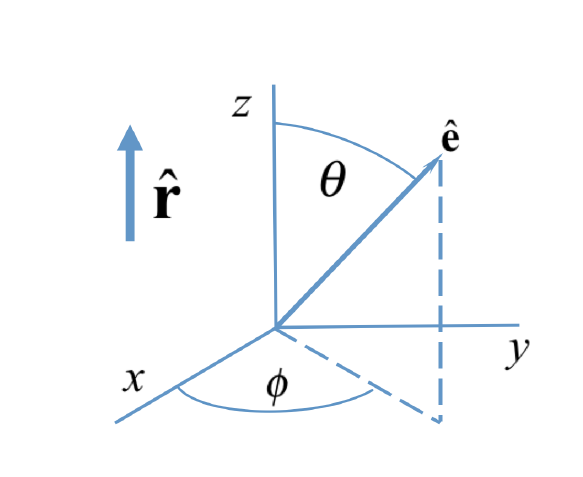
\includegraphics[scale=0.5]{coordinates.png}
\caption{\label{fig:coords}Coordinates describing dipole orientation $\hat{\bf e}$.  $z$ axis is defined to be parallel with $\hat{\bf r}$, the unit vector specifying the direction from one dipole to the other.}
\end{figure}

The weight function $p$ is defined as the Boltzmann factor for the pair:
\begin{subequations}
\begin{equation}
\label{eq:pdef}
p=\exp\left[-\beta( u_E + u_{DD}) \right]
\end{equation}
and $q$ is the integral over the mapping coordinates,
\begin{equation}
\label{eq:qdef}
q=\int_0^{2\pi} d\phi_1\int_0^{2\pi} d\phi_2 \int_{-1}^{1} d(\cos\theta_1) \int_{-1}^{1} d(\cos\theta_2) p(\theta_1,\theta_2,\phi_1,\phi_2).
\end{equation}
\end{subequations}

We consider mapping for $E_z$, $E_x$ and $E_y$ separately.  The full free-energy derivative will be obtained by summing these three terms. Let us start with $E_z$.  The mapping equation is
\begin{equation}
\label{eq:master1}
\frac{\partial }{\partial E_z}\left(\frac{p}{q}\right)+\nabla\cdot\left(\frac{p}{q}{\bf v}^{E_z}\right)=0;
\end{equation}
or, equivalently
\begin{equation}
\label{eq:master2}
\frac{\partial p}{\partial E_z}-\frac{p}{q}\frac{\partial q}{\partial E_z}+\nabla\cdot\left(p{\bf v}^{E_z}\right)=0.
\end{equation}
We note that
\begin{subequations}
\label{eq:pqDerivs}
\begin{align}
\label{eq:pDeriv}
\frac{\partial p}{\partial E_z}&=\beta\mu (\cos\theta_1 + \cos\theta_2)p \\
\label{eq:qDeriv}
\frac{\partial q}{\partial E_z}&=\beta\mu \int_0^{2\pi} d\phi_1\int_0^{2\pi} d\phi_2 \int_{-1}^{1} d(\cos\theta_1) \int_{-1}^{1} d(\cos\theta_2) (\cos\theta_1 + \cos\theta_2)p(\theta_1,\theta_2,\phi_1,\phi_2)
\end{align}
\end{subequations}
The divergence operator for these coordinates is written here for a general vector ${\bf A}$ defined in the $(\theta_1,\theta_2,\phi_1,\phi_2)$ space:
\begin{align}
\label{eq:divergence}
\nabla\cdot {\bf A} =& \frac{1}{\sin\theta_1}\frac{\partial}{\partial \theta_1}\left(A_{\theta_1} \sin\theta_1\right)+\frac{1}{\sin\theta_2}\frac{\partial}{\partial \theta_2}\left(A_{\theta_2} \sin\theta_2\right)\nonumber\\
& + \frac{1}{\sin\theta_1}\frac{\partial A_{\phi_1}}{\partial \phi_1} + \frac{1}{\sin\theta_2}\frac{\partial A_{\phi_2}}{\partial \phi_2}
\end{align}

In the present application, ${\bf A} = p {\bf v}^{E_z}$, and our aim is to evaluate the $(\theta_1,\theta_2,\phi_1,\phi_2)$ components of ${\bf v}^{E_z}$. The necessary ``initial condition'' is that ${\bf v}^{E_z}\equiv 0$ for $\theta_1 = \theta_2 = 0$. 

We can perhaps make progress by taking advantage of some features of the problem:
\begin{itemize}
\item The problem is underspecified, so we can satisfy \eqref{eq:master2} by separating it into parts involving only some of the variables, and solving these independently. We would aim to have a separate equation for each component of ${\bf v}^{E_z}$.
\item We need ${\bf v}^{E_z}$ and its $E_z$ derivative only for the limit $E_z\to0$, so we can expand $\exp(-\beta u_{\rm E})$ to say, second order (perhaps first is enough).
\item We can similarly expand $\exp(-\beta u_{\rm DD})$, considering that $r$ may be large, and $u_{\rm DD} = O(r^{-3})$. We would then generate a solution for ${\bf v}^{E_z}$ as a series in $1/r$. The first term should be the non-interacting result, Eq.~\eqref{eq:noninteractMap}.
\item We can try a solution in which we assume no mapping of $\phi_1, \phi_2$ ($A_{\phi_1} = A_{\phi_2} = 0$).  
\end{itemize}

\subsection{Poisson equation} 
We define $\psi(\theta_1,\theta_2)$ such that
\begin{subequations}
\label{eq:psiDef}
\begin{align}
&\frac{\partial \psi}{\partial \theta_1} = p {\bf v}^{E_z}_{\theta_1} \sin\theta_1\sin\theta_2\\
&\frac{\partial \psi}{\partial \theta_2} = p {\bf v}^{E_z}_{\theta_2} \sin\theta_1\sin\theta_2
\end{align}
\end{subequations}
Assume for now that ${\bf v}^{E_z}_{\phi_1} = {\bf v}^{E_z}_{\phi_2} = 0$. We multiply \eqref{eq:master2} through by $\sin\theta_1\sin\theta_2$, then in terms of $\psi$ we have a Poisson equation
\begin{align}
\frac{\partial^2 \psi}{\partial \theta_1^2} + \frac{\partial^2 \psi}{\partial \theta_2^2} &= \sin\theta_1\sin\theta_2 \left(-\frac{\partial p}{\partial E_z}+\frac{p}{q}\frac{\partial q}{\partial E_z}\right)\nonumber\\
&= p(\theta_1,\theta_2)\sin\theta_1\sin\theta_2 \left(-\beta\mu(\cos\theta_1+\cos\theta_2)+Q_z\right)
\end{align}
where $Q_z \equiv (1/q)\partial q/\partial E_z$, and depends only on $r$. Note that $p(\theta_1,\theta_2)$ is given by  \eqref{eq:energyFns} and \eqref{eq:pdef}.

What to do for boundary conditions?  From \eqref{eq:psiDef}, clearly we have $\partial\psi/\partial\theta_1 = \partial\psi/\partial\theta_2 = 0$ for $\theta_1$ or $\theta_2$ equal to 0 or $\pi$.  What else do we need?

\section{Heisenberg models}
The Heisenberg model is a lattice model similar to the Ising model, but with spins that take on a full range of orientations (rather than just `up' and `down'). Instead of \eqref{eq:dipoleDipole}, the potential is
\begin{subequations}
\label{eq:Heisenberg}
\begin{align}
&u_{\rm E}=-\mu {\bf E}\cdot \left({\hat {\bf e}}_{1}+ {\hat {\bf e}}_2 \right) \\ 
&u_{\rm DD}= -J\left({\hat {\bf e}}_{1}\cdot{\hat {\bf e}}_{2}\right),
\end{align}
\end{subequations}
where $J$ is the coupling constant.

\subsection{2 dimensions}
In 2D, the orientation is specified by the angle $\theta$, in which case \eqref{eq:Heisenberg} is
\begin{subequations}
\label{eq:Heisenberg2D}
\begin{align}
&u_{\rm E}=-\mu \left[E_x (\cos \theta_1 +\cos\theta_2) + E_y(\sin\theta_1+\sin\theta_2)\right]\\
&u_{\rm DD}= -J\cos(\theta_2-\theta_1).
\end{align}
\end{subequations}
Equation \eqref{eq:pdef} for $p$ is unchanged, but for $q$ we have
\begin{equation}
\label{eq:qdef2D}
q=\int_0^{2\pi} d\theta_1\int_0^{2\pi} d\theta_2 p(\theta_1,\theta_2),
\end{equation}
and in place of \eqref{eq:qDeriv} we have
\begin{subequations}
\begin{align}
\frac{\partial q}{\partial E_x}&=\beta\mu \int_0^{2\pi} d\theta_1\int_0^{2\pi} d\theta_2 (\cos\theta_1 + \cos\theta_2)p(\theta_1,\theta_2)\\
\frac{\partial q}{\partial E_y}&=\beta\mu \int_0^{2\pi} d\theta_1\int_0^{2\pi} d\theta_2 (\sin\theta_1 + \sin\theta_2)p(\theta_1,\theta_2)
\end{align}
\end{subequations}
Now the divergence operator is, in place of \eqref{eq:divergence}:
\begin{equation}
\label{eq:divergence2D}
\nabla\cdot {\bf A} =\frac{\partial A_{\theta_1}}{\partial \theta_1} + \frac{\partial A_{\theta_2}}{\partial \theta_2}
\end{equation}
with ${\bf A}$ representing $p{\bf v}^{E_x}$. The balance equation that we need to solve is, for $E_x$ mapping ($E_y$ mapping is similar, but with $\sin$ in place of $\cos$):
\begin{equation}
\label{eq:balance2D}
\frac{\partial A_{\theta_1}}{\partial \theta_1} + \frac{\partial A_{\theta_2}}{\partial \theta_2} = -\beta\mu(\cos\theta_1+\cos\theta_2)p + \frac{p}{q}\frac{\partial q}{\partial E_x}
\end{equation}
or, writing all $\theta$ dependences explicitly
\begin{equation}
\label{eq:balance2Dfull}
\frac{\partial A_{\theta_1}}{\partial \theta_1} + \frac{\partial A_{\theta_2}}{\partial \theta_2} = \left(-\beta\mu(\cos\theta_1+\cos\theta_2) + Q_x\right)e^{\beta J\cos(\theta_2-\theta_1)+\beta\mu E_x(\cos\theta_1+\cos\theta_2)}
\end{equation}
($Q_x$ is independent of $\theta_1$ and $\theta_2$). We can put this in the Poisson form by defining
\begin{subequations}
\label{eq:psiDef2}
\begin{align}
&\frac{\partial \psi}{\partial \theta_1} = A_{\theta_1} \\
&\frac{\partial \psi}{\partial \theta_2} = A_{\theta_2};
\end{align}
\end{subequations}
however, we do not have an explicit requirement for the boundary condition, compared to $\partial\psi/\partial\theta = 0, \theta = 0,\pi$ used above. We do still satisfy the requirement that the integral of the right-hand side of \eqref{eq:balance2Dfull} is zero. The boundary condition that we can specify \emph{a priori} is $A_{\theta_1} = A_{\theta_2} = 0$ when $\theta_1 = \theta_2 = 0$.

%We note that if we choose $A(\theta_1,\theta_2)$ of the form
%\begin{equation}
%A(\theta_1,\theta_2) = g(\theta_1,\theta_2) e^{-\beta J\cos(\theta_2-\theta_1)+\beta\mu E_x(\cos\theta_1+\cos\theta_2)}
%\end{equation}
%then we have for $g$
%\begin{equation}
%\frac{\partial g_{\theta_1}}{\partial \theta_1} + \frac{\partial g_{\theta_2}}{\partial \theta_2} =  \beta\mu E_x (\sin\theta_1+\sin\theta_2)g(\theta_1,\theta_2) + \left(\beta\mu(\cos\theta_1+\cos\theta_2) + Q_x\right)
%\end{equation}

As an aside, let us note that we can reformulate the balance equation to change how $p$ enters into it.  Going from \eqref{eq:master2}, we write
\begin{equation*}
\nabla\cdot{\bf v}^{E_x}+\frac{1}{p}{\bf v}^{E_x}\cdot\nabla p=-\frac{\partial \ln p}{\partial E_x}+Q_x(E_x).%\frac{1}{q}\frac{\partial q}{\partial E_x}.
\end{equation*}
\begin{equation}
\label{eq:master3}
\nabla\cdot{\bf v}^{E_x}+{\bf v}^{E_x}\cdot\nabla \ln p=-\frac{\partial \ln p}{\partial E_x}+Q_x(E_x).%\frac{1}{q}\frac{\partial q}{\partial E_x}.
\end{equation}
So, for example, \eqref{eq:balance2D} would become
\begin{align}
\label{eq:balance2D3}
\frac{\partial { v}^{E_x}_{\theta_1}}{\partial \theta_1} + \frac{\partial { v}^{E_x}_{\theta_2}}{\partial \theta_2} 
&- { v}^{E_x}_{\theta_1} [\beta\mu E_x \sin\theta_1 - \beta J \sin(\theta_2-\theta_1)]\nonumber\\
&- { v}^{E_x}_{\theta_2} [\beta\mu E_x \sin\theta_2 + \beta J \sin(\theta_2-\theta_1)]= -\beta\mu(\cos\theta_1+\cos\theta_2) + Q_x,
\end{align}
or, in terms of $\psi$
\begin{align}
\label{eq:balance2D4}
\frac{\partial^2 \psi}{\partial \theta_1} + \frac{\partial^2\psi }{\partial \theta_2} 
&- \frac{\partial \psi}{\partial \theta_1} [\beta\mu E_x \sin\theta_1 - \beta J \sin(\theta_2-\theta_1)]\nonumber\\
&- \frac{\partial \psi}{\partial\theta_2} [\beta\mu E_x \sin\theta_2 + \beta J \sin(\theta_2-\theta_1)]=- \beta\mu(\cos\theta_1+\cos\theta_2) + Q_x,
\end{align}

\subsubsection{Stream-function approach}
Alternatively, we define $\chi$ such that
\begin{subequations}
\label{eq:chiDef}
\begin{align}
&{ v}^{E_x}_{\theta_1}=\frac{\partial \chi}{\partial \theta_2}\\
&{ v}^{E_x}_{\theta_2}=-\frac{\partial \chi}{\partial \theta_1},
\end{align}
\end{subequations}
then for \eqref{eq:balance2D3} we have
\begin{align}
\label{eq:balance2Dchi}
- \frac{\partial \chi}{\partial \theta_2} [\beta\mu E_x \sin\theta_1 - \beta J \sin(\theta_2-\theta_1)]&+ \frac{\partial \chi}{\partial\theta_1} [\beta\mu E_x \sin\theta_2 + \beta J \sin(\theta_2-\theta_1)]\nonumber\\
&= -\beta\mu(\cos\theta_1+\cos\theta_2) + Q_x,
\end{align}
We cannot satisfy this equation in the limiting case of $\theta_1 = \theta_2 = 0$, where $v_{\theta_1} = v_{\theta_2} = 0$. Instead, we define
\begin{subequations}
\label{eq:chiDef2}
\begin{align}
&{ v}^{E_x}_{\theta_1}=\frac{\partial \chi}{\partial \theta_2}-\beta\mu\sin\theta_1 + \frac{1}{2}\theta_1 Q_x\\
&{ v}^{E_x}_{\theta_2}=-\frac{\partial \chi}{\partial \theta_1}-\beta\mu\sin\theta_2 + \frac{1}{2}\theta_2 Q_x,
\end{align}
\end{subequations}
then
\begin{align}
\label{eq:balance2Dchi2}
&\left(\frac{\partial \chi}{\partial \theta_2} -\beta\mu\sin\theta_1 + \frac{1}{2}\theta_1 Q_x\right)[\beta\mu E_x \sin\theta_1 - \beta J \sin(\theta_2-\theta_1)]\nonumber\\
&+ \left(-\frac{\partial \chi}{\partial\theta_1}-\beta\mu\sin\theta_2 + \frac{1}{2}\theta_2 Q_x\right) [\beta\mu E_x \sin\theta_2 + \beta J \sin(\theta_2-\theta_1)]\nonumber\\
&= 0
\end{align}
This can be rearranged to have the same form as \eqref{eq:balance2Dchi}, but with a different right-hand side.

\subsection{Back to 3D}
Here's a summary of how the equations are modified for the 3D case.
\begin{itemize}
\item Eq. \eqref{eq:master3} is still the starting point, but we need to interpret the $\nabla$ operator for 3D rotation, thus:
\begin{subequations}
\label{eq:del3D}
\begin{align}
&\nabla \ln p =\sum_{i=1}^2 \frac{\partial \ln p}{\partial \theta_i} \hat {\boldsymbol \theta}_i + \frac{1}{\sin\theta_i}\frac{\partial \ln p}{\partial \phi_i}\hat{\boldsymbol \phi_i}\\
&\nabla \cdot {\bf v} = \sum_{i=1}^2 \frac{1}{\sin\theta_i}\frac{\partial}{\partial \theta_i}({\bf v}_{\theta_i}\sin\theta_i) + \frac{1}{\sin\theta_i}\frac{\partial {\bf v}_{\phi_i}}{\partial \phi_i}
\end{align}
\end{subequations}
\item $\ln p = -\beta (u_{\rm E} + u_{\rm DD})$, where $u_{\rm E}$ and $u_{\rm DD}$ are given by Eq.~\eqref{eq:energyFns} rather than \eqref{eq:Heisenberg2D}.
\end{itemize}

This needs to be done for all three components, $E_x, E_y$, and $E_z$. As with the 2D case, we can treat these all independently, and focus on one at a time.  So as a start we can again aim to get solutions that are 0th and 1st order in $E_x$ while taking $E_y = E_z = 0$; then obtain analogous solutions likewise for $E_y$ and $E_z$ (actually $E_z$ might be simplest and most similar to 2D, so that would be the best place to start).

\end{document}  
